On considère cinq îlots colorés différemment que nous nommerons \quote{bases}. Chacune de ces bases contient deux trous pour y accueillir deux jetons.
Pour chaque couleur $\cal C$ sauf une, disons $\cal C^{\prime\prime}$, on a deux jetons de couleur $\cal C$.
Par contre, on a juste un jeton de couleur $\cal C^{\prime\prime}$.
La partie commence en mettant au hasard deux jetons sur chaque base sauf une qui ne contiendra qu'un seul jeton.
Voici un exemple où c'est le jeton noir qui est seul, et c'est sur la base bleue qu'il n'y a qu'un seul jeton.

\begin{center}   % [3, 1, 2, None, 3, 1, 4, 0, 4, 2]
    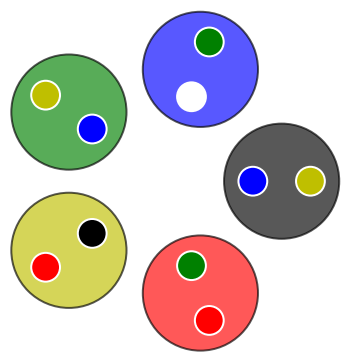
\includegraphics[scale= 0.3]{content/rules/start.png}
\end{center}

Le seul mouvement autorisé est le déplacement d'un jeton vers le trou libre à condition que le dit jeton et le trou soient dans des bases \quote{directement} voisines. Dans l'exemple ci-dessus, on ne peut donc bouger que l'un des jetons des bases bleue et rouge. Le but du jeu est d'obtenir la configuration suivante où chaque jeton a retrouvé sa base (la position du trou dans la base noire est sans importance).

\begin{center}
    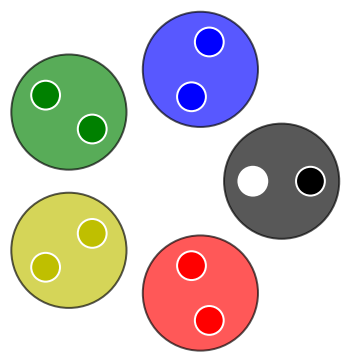
\includegraphics[scale= 0.3]{content/rules/end.png}
\end{center}

Si vous ne connaissez pas ce jeu nous vous conseillons, avant de lire la suite de ce document, d'essayer de trouver une méthode (il en existe plusieurs possibles et peut-être que vous trouverez d'autres points de vue que ceux que nous proposerons plus bas). Pour cela, il suffit d'expérimenter en vous fabriquant des bases et des jetons carrés, ce qui est très vite fait.


\paragraph{Remarque :} \hspace{-1em} dans ce jeu nous avons à tout moment accès à toutes les informations mais on pourrait très bien imaginer n'avoir accès qu'aux informations présentes sur trois bases voisines (concrètement, on mettrait les bases sur un plateau tournant avec au-dessus un cache ne laissant apparaître que trois bases). Il faut savoir qu'en informatique l'on peut avoir ce type de contrainte : par exemple, les routeurs qui dirigent les informations sur le réseau physique de l'internet n'ont pas une connaissance globale du réseau et pourtant ils arrivent à trouver d'assez bonnes solutions pour acheminer des données.
